% Informe de avance, semana 3. Compilar desde docs/ con:  xelatex informe_semana3.tex  (dos veces)
% Las tablas de informe_s2/ y las figuras fig/s2_*.png se generan con:  python docs/generar_informe_s2.py
\documentclass[11pt,letterpaper]{article}
\usepackage{amsmath,amssymb}
\usepackage{fontspec}
\setmainfont{TeX Gyre Termes}
\setmonofont[Scale=0.82]{Consolas}
\usepackage[spanish,es-noshorthands,es-tabla]{babel}
\usepackage[margin=2.3cm]{geometry}
\usepackage{longtable,booktabs,array}
\usepackage{graphicx}
\usepackage{xcolor}
\usepackage{caption}
\usepackage{enumitem}
\usepackage{fancyhdr}
\usepackage[hidelinks]{hyperref}
\definecolor{azul}{HTML}{1F3A5F}
\definecolor{fondo}{HTML}{EEF2F5}
\usepackage{titlesec}
\titleformat{\section}{\Large\bfseries\color{azul}}{\thesection}{1em}{}
\titleformat{\subsection}{\large\bfseries\color{azul}}{\thesubsection}{1em}{}
\setlength{\parskip}{5pt}
\setlength{\parindent}{0pt}
\setlength{\LTpre}{4pt}
\setlength{\LTpost}{4pt}
\setlist{itemsep=2pt,topsep=3pt}
\setlist[itemize]{label=$\bullet$}
\captionsetup{font=small,labelfont=bf}
\pagestyle{fancy}
\fancyhf{}
\fancyhead[L]{\small SIMTELE-RISK · Semana 3}
\fancyhead[R]{\small Métodos Numéricos · UMSA, FCPN}
\fancyfoot[C]{\small\thepage}
\renewcommand{\headrulewidth}{0pt}
\newcommand{\caja}[1]{\par\noindent\colorbox{fondo}{\parbox{\dimexpr\linewidth-2\fboxsep}{#1}}\par}

\begin{document}

% ---------------- Portada ----------------
\begin{titlepage}
\centering
{\large\bfseries UNIVERSIDAD MAYOR DE SAN ANDRÉS\par}
Facultad de Ciencias Puras y Naturales · Carrera de Informática\par
MÉTODOS NUMÉRICOS\par
\vspace{1.6cm}
{\fontsize{34}{40}\selectfont\bfseries\color{azul} SIMTELE-RISK\par}
\vspace{2pt}
Desafío integrador final\par
\vspace{1.2cm}

\includegraphics[height=6.2cm]{fig/logo_umsa.png}\par
\vspace{1.4cm}
{\large\bfseries Informe de avance, semana 3: integración matemática, aplicación y persistencia\par}
\vspace{0.4cm}
{\bfseries Integrantes\par}
\vspace{4pt}
{\small
\begin{tabular}{p{6.4cm}llp{3.4cm}}
\toprule
\textbf{Nombre} & \textbf{CI} & \textbf{RU} & \textbf{Mención}\\
\midrule
Saúl Walter Callisaya Sumi & 15074779 & 1885982 & Ingeniería de Sistemas\\
Ignacio Josue Zarate Camargo & 12392989 & 1886051 & IA y Ciencia de Datos\\
Luis Alejandro Zeballos Quiroz & 12896709 & 1886052 & IA y Ciencia de Datos\\
Jhoel Percy González Herrera & 9990880 & 1886116 & Ingeniería de Sistemas\\
\bottomrule
\end{tabular}\par}
\vfill
La Paz, Bolivia · noviembre de 2026
\end{titlepage}

\tableofcontents
\newpage

% ---------------- 1 ----------------
\section{Alcance entregado}
Este informe documenta la semana 3 de SIMTELE-RISK. Sobre los modelos, la teoría de errores y los sistemas lineales de la semana 1, se implementaron las familias de interpolación, raíces, integración y EDO; los cuatro módulos ejecutan sus \textbf{tres} escenarios (no sólo el NORMAL) con tablas, errores y al menos cuatro gráficos cada uno; la base de datos quedó conectada a una API y se comprobó el ciclo guardar → reiniciar → recuperar → repetir.

{\small
\begin{longtable}{p{6.0cm}p{2.6cm}p{6.6cm}}
\toprule
\textbf{Compromiso de la semana 3} & \textbf{Estado} & \textbf{Evidencia}\\
\midrule
Interpolación: Lagrange, Newton (diferencias divididas), spline cúbico & Hecho & Sección 3.1; \texttt{numerico/interpolacion.py}\\
Raíces: bisección, Newton-Raphson, secante & Hecho & Sección 3.2; \texttt{numerico/raices.py}\\
Integración: trapecio, Simpson 1/3, Romberg & Hecho & Sección 3.3; \texttt{numerico/integracion.py}\\
EDO: RK2 (Heun, variante declarada) y RK4 & Hecho & Sección 3.4; \texttt{numerico/edo.py}\\
Los 4 módulos ejecutan NORMAL con tablas, errores y 2 gráficos & Hecho (y además ESTRÉS y MAL COND.) & Sección 4; \texttt{casos/*.py}; 12 escenarios\\
Escenarios ESTRÉS y MAL CONDICIONADO y primeras comparaciones & Hecho & Secciones 4 y 5\\
Base de datos funcional; guardar y recuperar una ejecución & Hecho & Sección 6; \texttt{persistencia.py}, \texttt{api.py}\\
Enlace de la aplicación, repositorio e informe de experimentos y fallos & Hecho (enlace: ver sección 2.3) & Secciones 2 y 7\\
\bottomrule
\end{longtable}}

Las pruebas automáticas pasan de 21 (semana 1) a \textbf{54 superadas}: 22 de métodos con solución analítica, 10 de los 12 escenarios, persistencia y API, y 22 de la semana 1 (sistemas y esquema SQL, una nueva) (\texttt{backend/tests/} y \texttt{database/tests/}).

% ---------------- 2 ----------------
\section{Arquitectura de la aplicación}
\subsection{Componentes}
\begin{itemize}
\item \textbf{Núcleo numérico} (\texttt{backend/simtele/numerico/}): \texttt{errores}, \texttt{sistemas} (semana 1), \texttt{raices}, \texttt{integracion}, \texttt{edo}, \texttt{interpolacion}. Funciones puras que devuelven el valor, las iteraciones, si convergió y el criterio de parada.
\item \textbf{Casos de estudio} (\texttt{backend/simtele/casos/}): un archivo por módulo con sus parámetros validados (rango, tipo, opciones), los tres escenarios con su fuente de datos y la función \texttt{ejecutar}, que produce un \emph{resultado canónico}: indicadores, ejecuciones por método (iteraciones + resumen), tablas, gráficos y las dos conclusiones separadas.
\item \textbf{Persistencia} (\texttt{persistencia.py}, SQLite): traduce el resultado canónico al modelo relacional y lo reconstruye leyendo sólo la base.
\item \textbf{API REST} (\texttt{api.py}, FastAPI) y \textbf{aplicación web} (\texttt{frontend/}, HTML + JavaScript + Chart.js) servida por la misma API.
\end{itemize}

{\small
\begin{longtable}{p{5.6cm}p{9.6cm}}
\toprule
\textbf{Ruta} & \textbf{Función}\\
\midrule
\texttt{GET /api/modulos} & Modelos, parámetros con rangos y escenarios de los 4 módulos.\\
\texttt{POST /api/simular} & Valida, ejecuta y (opcionalmente) guarda una simulación. Parámetros inválidos → 422 con la lista de problemas.\\
\texttt{GET /api/simulaciones?q=\&modulo=\&tipo=} & Historial con búsqueda por texto, módulo y escenario, paginado.\\
\texttt{GET /api/simulaciones/\{id\}} & Recupera la simulación completa desde la base.\\
\texttt{POST /api/simulaciones/\{id\}/relanzar} & Repite el cálculo con los parámetros guardados y compara método a método.\\
\bottomrule
\end{longtable}}

\subsection{Pantallas}
\textbf{Inicio}: cuatro tarjetas (Detención, Deterioro, Oscilaciones, Sensores), el panel general de comparación de los 12 escenarios y la cobertura de métodos por módulo. \textbf{Módulo}: modelo, variables, hipótesis, selector NORMAL/ESTRÉS/MAL CONDICIONADO, formulario de parámetros con validación en el navegador y en el servidor, y resultados: indicadores, gráficos, tabla de métodos con su criterio de parada, tabla de iteraciones de cada método, tablas de refinamiento y la interpretación con la \emph{conclusión numérica} y la \emph{conclusión del problema} en tarjetas separadas. \textbf{Historial}: buscar, abrir, visualizar y relanzar una simulación guardada. Si la API no está disponible, la página funciona en \emph{modo estático} con los 12 escenarios precalculados en \texttt{frontend/datos/experimentos.json} (sin historial).

\subsection{Ejecución y enlace}
Desde la raíz del repositorio:
\begin{verbatim}
pip install -r backend/requirements.txt
python -m backend.simtele.experimentos      # 12 escenarios + datos del panel
python -m pytest                            # 54 pruebas
python -m uvicorn backend.simtele.api:app --port 8000
\end{verbatim}
y abrir \url{http://localhost:8000/}. El repositorio incluye \texttt{render.yaml} para publicar la API con la aplicación en un servicio web de Python.

\caja{\textbf{Enlace de la aplicación:} \texttt{[completar con la URL del despliegue]}\\
\textbf{Repositorio:} \url{https://github.com/Saul-C006/desafio-final-metodos}\\
Versión estática (sin historial), si se activa GitHub Pages:\ \texttt{https://saul-c006.github.io/desafio-final-metodos/frontend/}}

% ---------------- 3 ----------------
\section{Métodos implementados y pruebas analíticas}
Todas las familias usan las medidas de la semana 1: error absoluto, relativo (omitido cuando la referencia es nula, nunca se divide por cero), porcentual, residual, sensibilidad $\kappa_{\mathrm{rel}}=|\delta S/S|/|\delta E/E|$ y orden observado $p=\ln(e_h/e_{h/2})/\ln 2$.

\subsection{Interpolación}
Lagrange $p_n(t)=\sum_i y_i\prod_{j\ne i}\frac{t-t_j}{t_i-t_j}$; Newton $p_n(t)=f[t_0]+f[t_0,t_1](t-t_0)+\dots$, con $f[t_i,\dots,t_{i+k}]=\frac{f[t_{i+1},\dots,t_{i+k}]-f[t_i,\dots,t_{i+k-1}]}{t_{i+k}-t_i}$ y evaluación de Horner. Ambos construyen el mismo polinomio: su diferencia sólo es redondeo. Spline cúbico natural: los momentos $M_i=s''(t_i)$, con $M_0=M_n=0$, cumplen
\[ h_{i-1}M_{i-1}+2(h_{i-1}+h_i)M_i+h_iM_{i+1}=6\Big(\tfrac{y_{i+1}-y_i}{h_i}-\tfrac{y_i-y_{i-1}}{h_{i-1}}\Big), \]
un sistema tridiagonal simétrico y estrictamente diagonal dominante (por tanto SPD) que se resuelve con el \textbf{gradiente conjugado} de la semana 1 (y se contrasta con Gauss-Seidel, Jacobi y LU). El condicionamiento se mide con la constante de Lebesgue $\Lambda=\max_t\sum_i|L_i(t)|$, que acota la amplificación del ruido de los datos.

\textit{Pruebas:} reproducción exacta de un polinomio de grado 4; derivada de Newton; spline exacto para rectas y de orden 4 en $e^t$; sistema del spline SPD; Runge con $\Lambda>10^4$ en nodos uniformes y $\Lambda<3.5$ en Chebyshev.

\subsection{Raíces}
\begin{enumerate}
\item \textbf{Bisección}: exige $f(a)f(b)<0$; $c=a+(b-a)/2$; se conserva el subintervalo con cambio de signo; parada $(b-a)/2\le$ tol. Iteraciones $=\lceil\log_2((b-a)/\mathrm{tol})\rceil$.
\item \textbf{Newton-Raphson}: $x_{k+1}=x_k-f(x_k)/f'(x_k)$; parada $|x_{k+1}-x_k|\le$ tol; se detiene si $f'(x_k)=0$.
\item \textbf{Secante}: $x_{k+1}=x_k-f(x_k)\frac{x_k-x_{k-1}}{f(x_k)-f(x_{k-1})}$; misma parada; se detiene si la secante es horizontal.
\end{enumerate}
Cada iteración registra $x_k$, $|f(x_k)|$ (residual), el paso y el error real $|x_k-x^*|$. \textit{Pruebas:} $\sqrt2$ con la cota exacta de iteraciones de la bisección, convergencia cuadrática de Newton, razón $4/5$ de Newton en una raíz de multiplicidad 5 y detección de derivada nula.

\subsection{Integración}
Trapecio compuesto $T(h)=h[\tfrac12f_0+\sum f_i+\tfrac12f_n]$ ($O(h^2)$), Simpson 1/3 compuesto ($n$ par, $O(h^4)$; con $n$ impar el último tramo usa Simpson 3/8) y Romberg $R_{i,j}=R_{i,j-1}+\frac{R_{i,j-1}-R_{i-1,j-1}}{4^j-1}$ con parada $|R_{i,i}-R_{i-1,i-1}|\le$ tol, que reutiliza las evaluaciones del nivel anterior. Hay variantes sobre muestras equiespaciadas para integrar la salida de RK4; Romberg sobre muestras usa los trapecios con pasos $h\,2^j$ que caben en la malla. \textit{Pruebas:} órdenes 2 y 4 en $\int_0^\pi\sin t\,dt$, Simpson exacto para cúbicas, Romberg exacto para quínticas en a lo sumo 4 niveles.

\subsection{Ecuaciones diferenciales}
Variante de RK2 declarada: \textbf{método de Heun}, $k_1=f(t_n,y_n)$, $k_2=f(t_n+h,y_n+hk_1)$, $y_{n+1}=y_n+\tfrac h2(k_1+k_2)$. RK4 clásico, $y_{n+1}=y_n+\tfrac h6(k_1+2k_2+2k_3+k_4)$. Para el frenado se integra hasta el \emph{evento} $v=0$: cuando un paso cambia el signo de $v$, el último paso $h^*$ se obtiene resolviendo $g(h^*)=v(\Phi_{h^*}(y_n))=0$ con la secante. La estabilidad se juzga con el factor de amplificación $R(h\lambda)$ en el autovalor $\lambda$ del sistema lineal: Heun $R=1+z+z^2/2$, RK4 $R=\sum_{k=0}^4 z^k/k!$. \textit{Pruebas:} órdenes 2 y 4 en $x''=-4x$, exactitud de ambos con desaceleración constante, evento $v=0$ y crecimiento espurio de Heun con $h=0.5$.

% ---------------- 4 ----------------
\section{Resultados por módulo y escenario}
Los parámetros de cada escenario son sintéticos y se declaran con su fuente. Las tablas de este apartado se generan con \texttt{python docs/generar\_informe\_s2.py} a partir de las mismas funciones que usa la aplicación; las iteraciones completas se ven en la aplicación y quedan guardadas en la base.

% ---- M1 ----
\subsection{Módulo 1: detención de emergencia}
Modelo: $\dot x=v$, $\dot v=-a(v,t)$, $x(0)=0$, $v(0)=v_0$, $d_{\mathrm{total}}=v_0t_r+x(t_{\mathrm{det}})$. Referencias cerradas: NORMAL ($a=a_0$) $t_{\mathrm{det}}=v_0/a_0$, $d=v_0^2/(2a_0)$; ESTRÉS ($a=a_0+c_2v^2$) $v(t)=s\tan(\varphi-kt)$ con $s=\sqrt{a_0/c_2}$, $k=\sqrt{a_0c_2}$, $t_{\mathrm{det}}=\varphi/k$, $d=\ln(1+c_2v_0^2/a_0)/(2c_2)$; MAL COND. $v=v_0(1-t/T)^5$, $t_{\mathrm{det}}=T$, $d=v_0T/6$. Métodos: Heun y RK4 (EDO con evento), bisección, Newton y secante para $v(t)=0$, trapecio, Simpson y Romberg para $\int_0^{t_{\mathrm{det}}}v\,dt$.

{\footnotesize
\begin{longtable}{lrrr}
\toprule
\textbf{Parámetro} & \textbf{NORMAL} & \textbf{ESTRÉS} & \textbf{MAL COND.} \\
\midrule
\endhead
Velocidad inicial v$_{0}$ [m/s] & 5 & 7 & 5 \\
Desaceleración base a$_{0}$ [m/s$^{2}$] & 2.5 & 1.2 & — \\
Coef. resistencia c$_{2}$ (a = a$_{0}$ + c$_{2}$v$^{2}$) [1/m] & 0 & 0.05 & — \\
Duración del frenado plano T [s] & — & — & 4 \\
Tiempo de reacción t\_r [s] & 0.5 & 1.5 & 0.5 \\
Paso de la EDO h [s] & 0.1 & 0.5 & 0.1 \\
Tolerancia de raíces & 1.000$\times10^{-10}$ & 1.000$\times10^{-13}$ & 1.000$\times10^{-10}$ \\
Distancia disponible [m] & 10 & 20 & 15 \\
\bottomrule
\end{longtable}
}

\textbf{Tabla de errores por método y escenario} (resultado: $d_{\mathrm{fren}}$ en m para EDO e integración; $t_{\mathrm{det}}$ en s para raíces):
{\footnotesize
\begin{longtable}{lllrlrrr}
\toprule
\textbf{Escenario} & \textbf{Familia} & \textbf{Método} & \textbf{Iter./pasos} & \textbf{Conv.} & \textbf{Resultado} & \textbf{Error abs.} & \textbf{Error rel. / otro} \\
\midrule
\endhead
NORMAL & EDO & Heun (RK2) & 20 & sí & 5 & 8.882$\times10^{-16}$ & 1.776$\times10^{-16}$ \\
NORMAL & EDO & RK4 & 20 & sí & 5 & 8.882$\times10^{-16}$ & 1.776$\times10^{-16}$ \\
NORMAL & Raíces & Bisección & 32 & sí & 2 & 2.328$\times10^{-11}$ & res. 5.821$\times10^{-11}$ \\
NORMAL & Raíces & Newton-Raphson & 2 & sí & 2 & 0 & res. 0 \\
NORMAL & Raíces & Secante & 1 & sí & 2 & 0 & res. 0 \\
NORMAL & Integración & Trapecio compuesto & 8 & sí & 5 & 0 & 0 \\
NORMAL & Integración & Simpson 1/3 compuesto & 8 & sí & 5 & 8.882$\times10^{-16}$ & 1.776$\times10^{-16}$ \\
NORMAL & Integración & Romberg & 2 & sí & 5 & 0 & 0 \\
ESTRÉS & EDO & Heun (RK2) & 8 & sí & 11.042119 & 0.0819 & 0.00737 \\
ESTRÉS & EDO & RK4 & 8 & sí & 11.123462 & 5.946$\times10^{-4}$ & 5.345$\times10^{-5}$ \\
ESTRÉS & Raíces & Bisección & 42 & sí & 3.9198703 & 5.640$\times10^{-14}$ & res. 6.799$\times10^{-14}$ \\
ESTRÉS & Raíces & Newton-Raphson & 6 & sí & 3.9198703 & 0 & res. 0 \\
ESTRÉS & Raíces & Secante & 6 & sí & 3.9198703 & 0 & res. 0 \\
ESTRÉS & Integración & Trapecio compuesto & 8 & sí & 11.124104 & 4.787$\times10^{-5}$ & 4.303$\times10^{-6}$ \\
ESTRÉS & Integración & Simpson 1/3 compuesto & 8 & sí & 11.124056 & 9.090$\times10^{-10}$ & 8.171$\times10^{-11}$ \\
ESTRÉS & Integración & Romberg & 9 & sí & 11.124056 & 1.776$\times10^{-15}$ & 1.597$\times10^{-16}$ \\
MAL COND. & EDO & Heun (RK2) & 30 & sí & 3.3117154 & 0.0216 & 0.00649 \\
MAL COND. & EDO & RK4 & 39 & sí & 3.3333325 & 8.055$\times10^{-7}$ & 2.417$\times10^{-7}$ \\
MAL COND. & Raíces & Bisección & 32 & sí & 4 & 2.328$\times10^{-11}$ & res. 3.341$\times10^{-56}$ \\
MAL COND. & Raíces & Newton-Raphson & 104 & sí & 4 & 3.337$\times10^{-10}$ & res. 2.022$\times10^{-50}$ \\
MAL COND. & Raíces & Secante & 146 & sí & 4 & 5.614$\times10^{-10}$ & res. 2.723$\times10^{-49}$ \\
MAL COND. & Integración & Trapecio compuesto & 8 & sí & 3.3334605 & 1.272$\times10^{-4}$ & 3.815$\times10^{-5}$ \\
MAL COND. & Integración & Simpson 1/3 compuesto & 8 & sí & 3.3333333 & 1.552$\times10^{-9}$ & 4.657$\times10^{-10}$ \\
MAL COND. & Integración & Romberg & 4 & sí & 3.3333333 & 0 & 0 \\
\bottomrule
\end{longtable}
}


\begin{figure}[h]\centering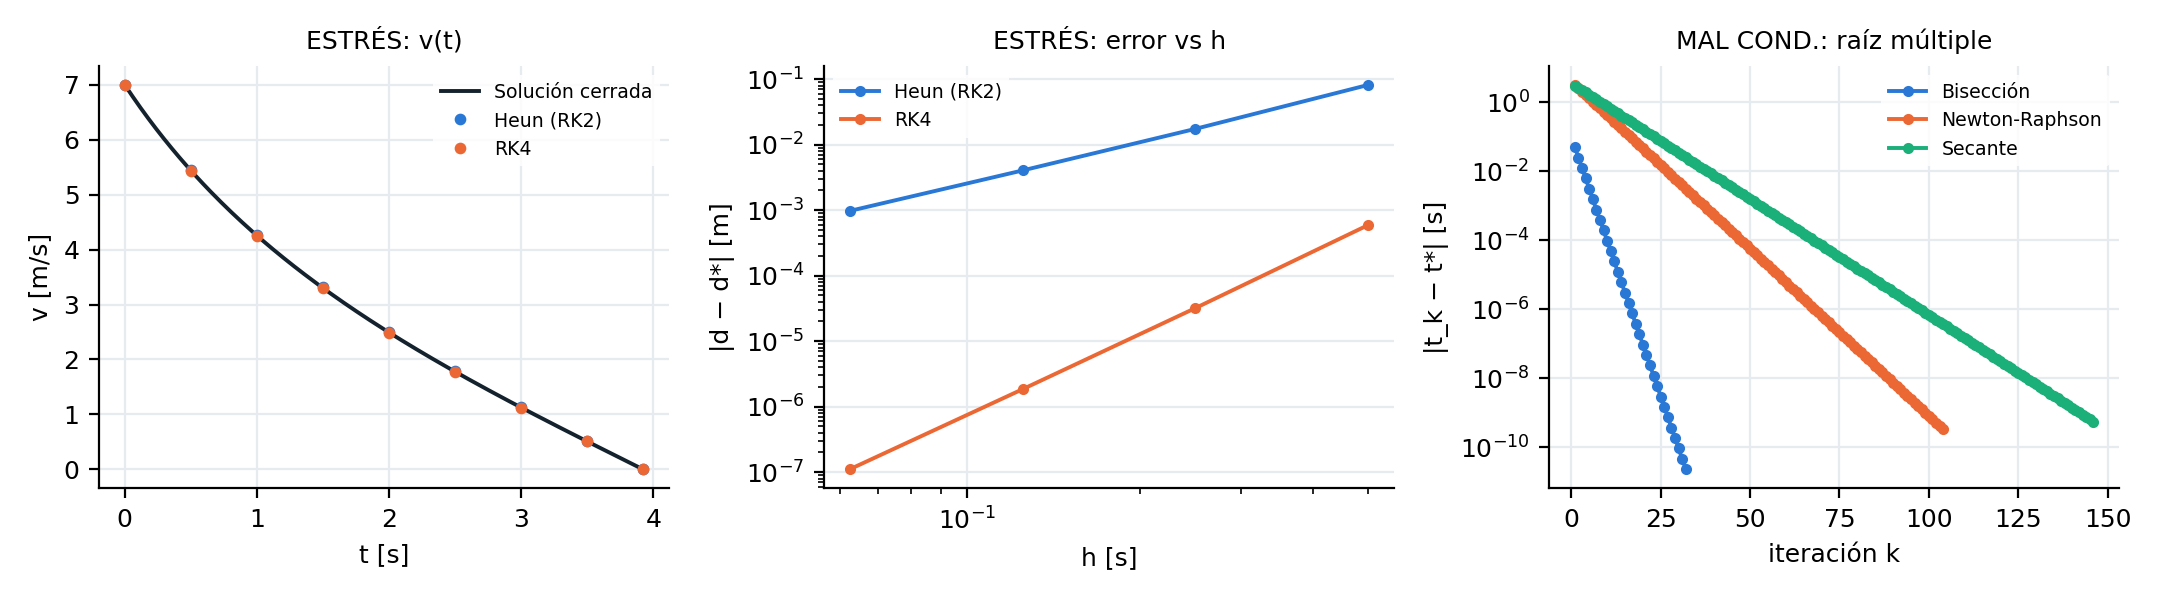
\includegraphics[width=\linewidth]{fig/s2_m1.png}
\caption{Módulo 1. Izquierda: velocidad en ESTRÉS con $h=0.5$ s. Centro: error en la distancia al refinar $h$ (pendientes 2 y 4). Derecha: convergencia de las raíces en la raíz múltiple: Newton y secante se vuelven lineales.}\end{figure}

\textbf{ESTRÉS, refinamiento del paso} (órdenes observados $\to2$ y $\to4$):
{\footnotesize
\begin{longtable}{lrrrrr}
\toprule
\textbf{Método} & \textbf{h [s]} & \textbf{|t\_det $-$ t*| [s]} & \textbf{orden p (t)} & \textbf{|d $-$ d*| [m]} & \textbf{orden p (d)} \\
\midrule
\endhead
Heun (RK2) & 0.5 & 0.00363436 & — & 0.0819372 & — \\
Heun (RK2) & 0.25 & 0.0011045 & 1.72 & 0.017471 & 2.23 \\
Heun (RK2) & 0.125 & 2.825$\times10^{-4}$ & 1.97 & 0.00404844 & 2.11 \\
Heun (RK2) & 0.0625 & 7.113$\times10^{-5}$ & 1.99 & 9.752$\times10^{-4}$ & 2.05 \\
RK4 & 0.5 & 2.918$\times10^{-5}$ & — & 5.946$\times10^{-4}$ & — \\
RK4 & 0.25 & 1.128$\times10^{-6}$ & 4.69 & 3.207$\times10^{-5}$ & 4.21 \\
RK4 & 0.125 & 5.200$\times10^{-8}$ & 4.44 & 1.849$\times10^{-6}$ & 4.12 \\
RK4 & 0.0625 & 2.742$\times10^{-9}$ & 4.25 & 1.109$\times10^{-7}$ & 4.06 \\
\bottomrule
\end{longtable}
}

\textbf{MAL CONDICIONADO, refinamiento del paso.} El error en $t_{\mathrm{det}}$ converge con orden $p/5$ (0.4 para Heun y 0.8 para RK4) mientras el error en la distancia conserva el orden 4 de RK4: el instante de detención es una raíz de multiplicidad 5 y un error $\varepsilon$ en $v$ lo desplaza $T(\varepsilon/v_0)^{1/5}$.
{\footnotesize
\begin{longtable}{lrrrrr}
\toprule
\textbf{Método} & \textbf{h [s]} & \textbf{|t\_det $-$ t*| [s]} & \textbf{orden p (t)} & \textbf{|d $-$ d*| [m]} & \textbf{orden p (d)} \\
\midrule
\endhead
Heun (RK2) & 0.1 & 1.00953 & — & 0.0216179 & — \\
Heun (RK2) & 0.05 & 0.766536 & 0.397 & 0.0056751 & 1.93 \\
Heun (RK2) & 0.025 & 0.581437 & 0.399 & 0.0014696 & 1.95 \\
Heun (RK2) & 0.0125 & 0.440808 & 0.399 & 3.770$\times10^{-4}$ & 1.96 \\
RK4 & 0.1 & 0.109965 & — & 8.055$\times10^{-7}$ & — \\
RK4 & 0.05 & 0.0633261 & 0.796 & 5.057$\times10^{-8}$ & 3.99 \\
RK4 & 0.025 & 0.0364465 & 0.797 & 3.169$\times10^{-9}$ & 4 \\
RK4 & 0.0125 & 0.0209596 & 0.798 & 1.983$\times10^{-10}$ & 4 \\
\bottomrule
\end{longtable}
}

{\footnotesize
\begin{longtable}{lrrrrr}
\toprule
\textbf{Método} & \textbf{t\_det [s]} & \textbf{Iteraciones} & \textbf{|t $-$ t*| [s]} & \textbf{|v(t)| residual} & \textbf{Orden observado} \\
\midrule
\endhead
Bisección & 3.99999999998 & 32 & 2.328$\times10^{-11}$ & 3.341$\times10^{-56}$ & 1 \\
Newton-Raphson & 3.99999999967 & 104 & 3.337$\times10^{-10}$ & 2.022$\times10^{-50}$ & 1 \\
Secante & 3.99999999944 & 146 & 5.614$\times10^{-10}$ & 2.723$\times10^{-49}$ & 1 \\
\bottomrule
\end{longtable}
}

\textbf{MAL CONDICIONADO, integración de un polinomio de grado 5}: trapecio orden 2, Simpson orden 4 y Romberg exacto.
{\footnotesize
\begin{longtable}{lrrrrrrr}
\toprule
\textbf{n} & \textbf{h [s]} & \textbf{Trapecio [m]} & \textbf{Error} & \textbf{orden} & \textbf{Simpson 1/3 [m]} & \textbf{Error} & \textbf{orden} \\
\midrule
\endhead
2 & 2 & 5.31249999998 & 1.97917 & — & 3.74999999999 & 0.416667 & — \\
4 & 1 & 3.84765624999 & 0.514323 & 1.94 & 3.359375 & 0.0260417 & 4 \\
8 & 0.5 & 3.46313476562 & 0.129801 & 1.99 & 3.3349609375 & 0.0016276 & 4 \\
16 & 0.25 & 3.36585998535 & 0.0325267 & 2 & 3.33343505859 & 1.017$\times10^{-4}$ & 4 \\
32 & 0.125 & 3.34146976471 & 0.00813643 & 2 & 3.33333969116 & 6.358$\times10^{-6}$ & 4 \\
64 & 0.0625 & 3.3353677392 & 0.00203441 & 2 & 3.3333337307 & 3.974$\times10^{-7}$ & 4 \\
128 & 0.03125 & 3.33384195343 & 5.086$\times10^{-4}$ & 2 & 3.33333335817 & 2.484$\times10^{-8}$ & 4 \\
256 & 0.015625 & 3.33346048952 & 1.272$\times10^{-4}$ & 2 & 3.33333333489 & 1.552$\times10^{-9}$ & 4 \\
\bottomrule
\end{longtable}
}

\textbf{Sensibilidad física (NORMAL)}:
{\footnotesize
\begin{longtable}{lrrrrrr}
\toprule
\textbf{Parámetro} & \textbf{Valor} & \textbf{Perturbado} & \textbf{d\_total [m]} & \textbf{d\_total' [m]} & \textbf{$\Delta$d [m]} & \textbf{$\kappa$\_rel} \\
\midrule
\endhead
v0 & 5 & 5.05 & 7.5 & 7.6255 & 0.1255 & 1.673 \\
tr & 0.5 & 0.505 & 7.5 & 7.525 & 0.025 & 0.3333 \\
a0 & 2.5 & 2.525 & 7.5 & 7.450495 & -0.049505 & 0.6601 \\
\bottomrule
\end{longtable}
}

\textbf{Primeras conclusiones.}
\begin{itemize}
\item \textbf{NORMAL.} \emph{Numérica:} Con desaceleración constante v(t) es lineal y x(t) cuadrática: Heun y RK4 reproducen la solución hasta el redondeo (error en d: 8.882$\times10^{-16}$ y 8.882$\times10^{-16}$ m), trapecio y Simpson son exactos y Newton y secante terminan en 2 y 1 iteraciones, frente a 32 de la bisección. Es un caso de verificación, no de comparación de órdenes. \emph{Problema:} La cabina se detiene en 7.5 m, con un margen de 2.5 m respecto a los 10 m disponibles. De ese total, 2.5 m se recorren durante la reacción. La distancia total es más sensible a v$_{0}$: $\kappa$\_rel = 1.673 para v$_{0}$ y 0.3333 para t\_r.
\item \textbf{ESTRÉS.} \emph{Numérica:} Con resistencia cuadrática y h = 0.5 s, Heun comete 0.0819372 m de error en la distancia y RK4 5.946$\times10^{-4}$ m; al refinar el paso los órdenes observados se acercan a 2 y 4. Newton converge cuadráticamente (6 iteraciones), la secante superlinealmente (6) y la bisección linealmente (42). Romberg alcanza la tolerancia con muchas menos evaluaciones que el trapecio. \emph{Problema:} La cabina necesita 21.62 m y excede en 1.62 m la distancia disponible de 20 m. De ese total, 10.5 m se recorren durante la reacción. La distancia total es más sensible a v$_{0}$: $\kappa$\_rel = 1.105 para v$_{0}$ y 0.4856 para t\_r.
\item \textbf{MAL COND..} \emph{Numérica:} La raíz t = T tiene multiplicidad 5: Newton pierde la convergencia cuadrática y avanza con razón 4/5 (104 iteraciones), la secante también se vuelve lineal (146) y el residuo |v(t)| es muchísimo menor que el error en t. Un desplazamiento de 1$\times10^{-12}$ m/s en v mueve la raíz 0.0115416 s (amplificación 1.154$\times10^{10}$): es mal condicionamiento del problema, no fallo de convergencia, porque los tres métodos sí convergen. El t\_det de las EDO tiene un error de 0.109965 s con RK4 aunque la distancia es precisa. \emph{Problema:} La cabina se detiene en 5.833 m, con un margen de 9.17 m respecto a los 15 m disponibles. De ese total, 2.5 m se recorren durante la reacción. La distancia total es más sensible a v$_{0}$: $\kappa$\_rel = 1 para v$_{0}$ y 0.4286 para t\_r. En el frenado plano el instante exacto de detención está mal definido (la cabina «se arrastra» al final), pero la distancia sí es confiable.
\end{itemize}


% ---- M2 ----
\subsection{Módulo 2: deterioro y mantenimiento}
Modelo: $D(t)=D_0+\alpha t+\beta t^2$, $f(t)=D(t)-D_u$. Referencia: menor raíz no negativa de la cuadrática calculada con 50 dígitos decimales y la fórmula sin cancelación $q=-\tfrac12\big(\alpha+\operatorname{sgn}(\alpha)\sqrt{\alpha^2-4\beta(D_0-D_u)}\big)$, $t\in\{q/\beta,\,(D_0-D_u)/q\}$. El intervalo de bisección se obtiene por búsqueda incremental de 1 mes. La calibración por tramos $A\mathbf x=\mathbf b$ de la semana 1 queda integrada al módulo con los mismos resultados. MAL COND.: $D(t)=40+10^{-6}-0.05(t-24)^2$, cuyo máximo queda $10^{-6}$ \% sobre el umbral, y la matriz de Hilbert $n=8$.

{\footnotesize
\begin{longtable}{lrrr}
\toprule
\textbf{Parámetro} & \textbf{NORMAL} & \textbf{ESTRÉS} & \textbf{MAL COND.} \\
\midrule
\endhead
Deterioro inicial D$_{0}$ [\%] & 10 & 25 & 11.200001 \\
Tasa lineal $\alpha$ [\%/mes] & 0.8 & 2 & 2.4 \\
Aceleración $\beta$ [\%/mes$^{2}$] & 0.02 & 0.15 & -0.05 \\
Umbral de inspección D\_u [\%] & 40 & 40 & 40 \\
Tolerancia de raíces & 1.000$\times10^{-10}$ & 1.000$\times10^{-13}$ & 1.000$\times10^{-10}$ \\
Retraso de mantenimiento [meses] & 3 & 3 & 3 \\
Matriz de calibración & tramos & tramos & hilbert \\
Tamaño del sistema n & 6 & 40 & 8 \\
Acoplamiento $\lambda$ (A = I + $\lambda$L) & 0.1 & 5 & 0 \\
Tolerancia de los iterativos & 1.000$\times10^{-10}$ & 1.000$\times10^{-12}$ & 1.000$\times10^{-10}$ \\
\bottomrule
\end{longtable}
}

\textbf{Tabla de errores por método y escenario} (raíces: $t^*$ en meses; sistemas: error de $\mathbf x$ y residuo relativo):
{\footnotesize
\begin{longtable}{lllrlrrr}
\toprule
\textbf{Escenario} & \textbf{Familia} & \textbf{Método} & \textbf{Iter./pasos} & \textbf{Conv.} & \textbf{Resultado} & \textbf{Error abs.} & \textbf{Error rel. / otro} \\
\midrule
\endhead
NORMAL & Raíces & Bisección & 34 & sí & 23.588989 & 2.661$\times10^{-12}$ & res. 4.640$\times10^{-12}$ \\
NORMAL & Raíces & Newton-Raphson & 6 & sí & 23.588989 & 0 & res. 0 \\
NORMAL & Raíces & Secante & 8 & sí & 23.588989 & 0 & res. 0 \\
NORMAL & Sistemas lineales & Jacobi & 13 & sí & — & 1.106$\times10^{-9}$ & res. 2.127$\times10^{-11}$ \\
NORMAL & Sistemas lineales & Gauss-Seidel & 8 & sí & — & 1.570$\times10^{-9}$ & res. 3.169$\times10^{-11}$ \\
NORMAL & Sistemas lineales & LU con pivoteo parcial & 1 & sí & — & 7.944$\times10^{-15}$ & res. 9.584$\times10^{-17}$ \\
NORMAL & Sistemas lineales & Gradiente conjugado & 5 & sí & — & 8.140$\times10^{-15}$ & res. 1.728$\times10^{-16}$ \\
ESTRÉS & Raíces & Bisección & 44 & sí & 5.3518376 & 3.730$\times10^{-14}$ & res. 1.350$\times10^{-13}$ \\
ESTRÉS & Raíces & Newton-Raphson & 6 & sí & 5.3518376 & 8.882$\times10^{-16}$ & res. 0 \\
ESTRÉS & Raíces & Secante & 7 & sí & 5.3518376 & 8.882$\times10^{-16}$ & res. 0 \\
ESTRÉS & Sistemas lineales & Jacobi & 285 & sí & — & 1.326$\times10^{-10}$ & res. 9.799$\times10^{-13}$ \\
ESTRÉS & Sistemas lineales & Gauss-Seidel & 147 & sí & — & 1.146$\times10^{-10}$ & res. 8.488$\times10^{-13}$ \\
ESTRÉS & Sistemas lineales & LU con pivoteo parcial & 1 & sí & — & 2.562$\times10^{-14}$ & res. 8.899$\times10^{-16}$ \\
ESTRÉS & Sistemas lineales & Gradiente conjugado & 22 & sí & — & 3.398$\times10^{-14}$ & res. 2.044$\times10^{-15}$ \\
MAL COND. & Raíces & Bisección & 34 & sí & 23.995528 & 2.626$\times10^{-11}$ & res. 7.105$\times10^{-15}$ \\
MAL COND. & Raíces & Newton-Raphson & 17 & sí & 23.995528 & 2.945$\times10^{-12}$ & res. 0 \\
MAL COND. & Raíces & Secante & 24 & sí & 23.995528 & 1.626$\times10^{-11}$ & res. 7.105$\times10^{-15}$ \\
MAL COND. & Sistemas lineales & Jacobi & 128 & no & — & 3.426$\times10^{100}$ & res. 9.076$\times10^{99}$ \\
MAL COND. & Sistemas lineales & Gauss-Seidel & 5000 & no & — & 0.0335 & res. 2.185$\times10^{-7}$ \\
MAL COND. & Sistemas lineales & LU con pivoteo parcial & 1 & sí & — & 3.394$\times10^{-7}$ & res. 2.677$\times10^{-17}$ \\
MAL COND. & Sistemas lineales & Gradiente conjugado & 8 & sí & — & 4.236$\times10^{-4}$ & res. 6.903$\times10^{-11}$ \\
\bottomrule
\end{longtable}
}


\begin{figure}[h]\centering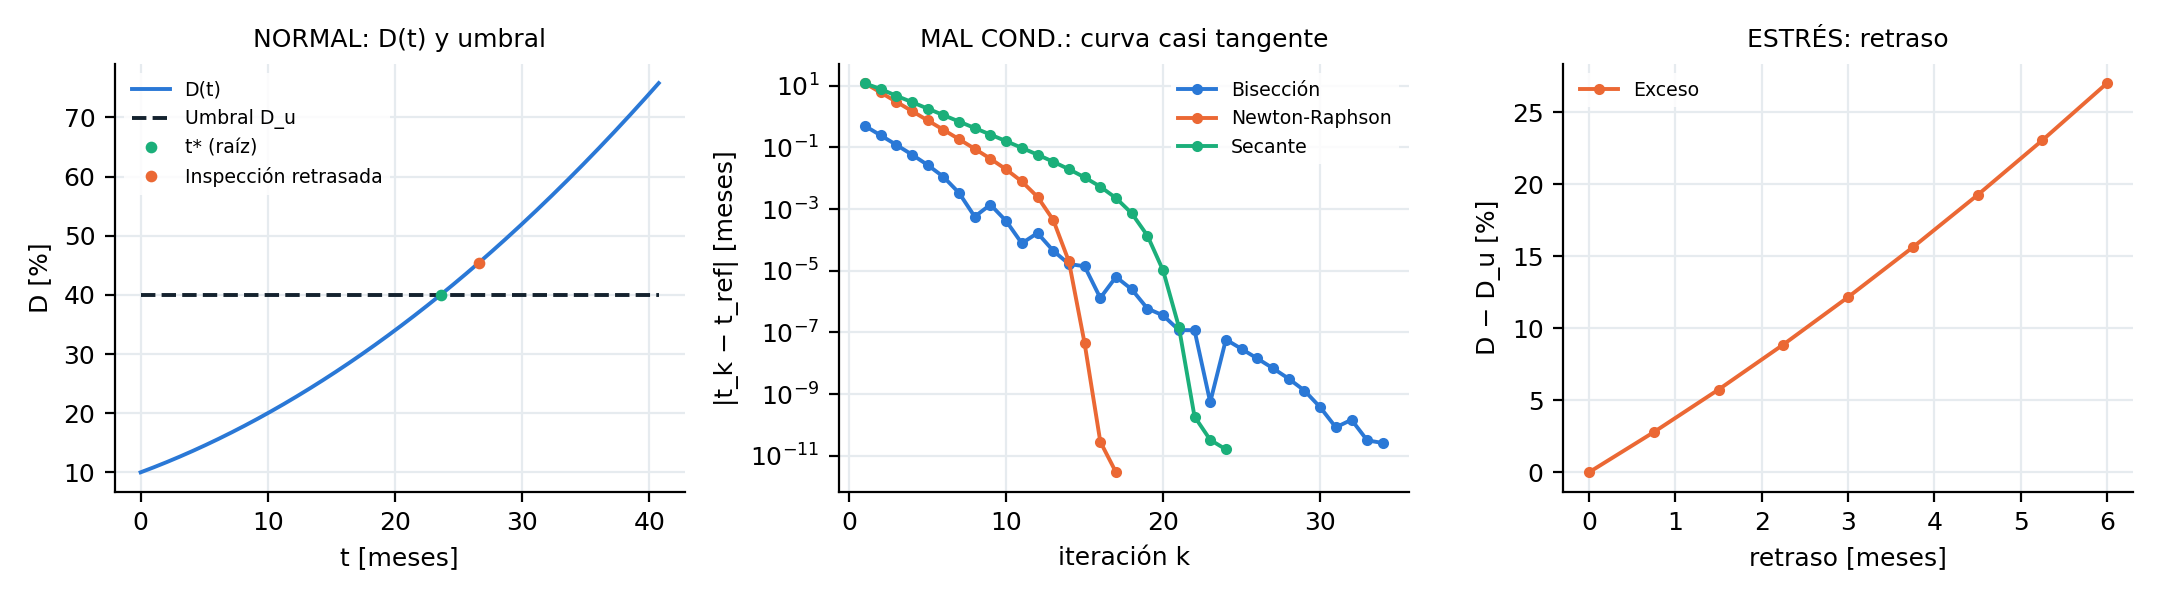
\includegraphics[width=\linewidth]{fig/s2_m2.png}
\caption{Módulo 2. Izquierda: indicador y umbral (NORMAL). Centro: convergencia de las raíces con la curva casi tangente. Derecha: exceso de deterioro según el retraso del mantenimiento (ESTRÉS).}\end{figure}

\textbf{Iteraciones de Newton (NORMAL)}:
{\footnotesize
\begin{longtable}{lrrrr}
\toprule
\textbf{k} & \textbf{t\_k} & \textbf{f(t\_k)} & \textbf{|t\_k $-$ t\_(k$-$1)|} & \textbf{|t\_k $-$ t\_ref|} \\
\midrule
\endhead
1 & 37.5 & 28.125 & 37.5 & 13.911 \\
2 & 25.271739130435 & 2.99061 & 12.2283 & 1.68275 \\
3 & 23.62026332272 & 0.0545474 & 1.65148 & 0.0312739 \\
4 & 23.589000646435 & 1.955$\times10^{-5}$ & 0.0312627 & 1.121$\times10^{-5}$ \\
5 & 23.588989435408 & 2.508$\times10^{-12}$ & 1.121$\times10^{-5}$ & 1.439$\times10^{-12}$ \\
6 & 23.588989435407 & 0 & 1.439$\times10^{-12}$ & 0 \\
\bottomrule
\end{longtable}
}

\textbf{Sensibilidad en el escenario MAL CONDICIONADO.} $D'(t^*)=4.47\times10^{-4}$ \%/mes da $\kappa=|D_u/(t^*D'(t^*))|\approx3.7\times10^3$; el valor medido con $+10^{-9}$ coincide. Con $+10^{-7}$ el umbral deja de alcanzarse: un cambio cualitativo. Los tres métodos convergen; lo mal condicionado es el problema.
{\footnotesize
\begin{longtable}{lrrrrr}
\toprule
\textbf{Parámetro} & \textbf{Perturbación} & \textbf{t* [meses]} & \textbf{t*' [meses]} & \textbf{$\Delta$t} & \textbf{$\kappa$\_rel medido} \\
\midrule
\endhead
Du & +1$\times10^{-9}$ relativo & 23.99552786 & 23.99561822 & 9.036$\times10^{-5}$ & 3766 \\
Du & +1$\times10^{-7}$ relativo & 23.99552786 & sin raíz: el umbral ya no se alcanza & — & $\infty$ (cambio cualitativo) \\
Du & +0.01 relativo & 23.99552786 & sin raíz: el umbral ya no se alcanza & — & $\infty$ (cambio cualitativo) \\
alfa & +0.01 relativo & 23.99552786 & 20.83740981 & -3.15812 & 13.16 \\
beta & +0.01 relativo & 23.99552786 & sin raíz: el umbral ya no se alcanza & — & $\infty$ (cambio cualitativo) \\
\bottomrule
\end{longtable}
}

\textbf{Primeras conclusiones.}
\begin{itemize}
\item \textbf{NORMAL.} \emph{Numérica:} Newton (6 iteraciones) y secante (8) alcanzan la raíz de referencia hasta el redondeo; la bisección necesita 34 iteraciones porque reduce el intervalo a la mitad en cada paso. En el sistema ($\kappa_{2}$ = 1.373), Gauss-Seidel requiere 8 iteraciones frente a 13 de Jacobi ($\rho$\_GS $\approx$ $\rho$\_J$^{2}$) y el gradiente conjugado 5; LU es exacto hasta el redondeo. \emph{Problema:} El indicador alcanza el umbral de 40 \% a los 23.589 meses. Un retraso de 3 meses lleva el desgaste a 45.411 \% (5.41 \% respecto del umbral; negativo indica que la curva ya volvió a bajar). La fecha es más sensible al umbral y a la tasa $\alpha$ cuanto menor es la pendiente D$'$(t*) = 1.744 \%/mes.
\item \textbf{ESTRÉS.} \emph{Numérica:} Newton (6 iteraciones) y secante (7) alcanzan la raíz de referencia hasta el redondeo; la bisección necesita 44 iteraciones porque reduce el intervalo a la mitad en cada paso. En el sistema ($\kappa_{2}$ = 20.97), Gauss-Seidel requiere 147 iteraciones frente a 285 de Jacobi ($\rho$\_GS $\approx$ $\rho$\_J$^{2}$) y el gradiente conjugado 22; LU es exacto hasta el redondeo. \emph{Problema:} El indicador alcanza el umbral de 40 \% a los 5.3518 meses. Un retraso de 3 meses lleva el desgaste a 52.167 \% (12.2 \% respecto del umbral; negativo indica que la curva ya volvió a bajar). La fecha es más sensible al umbral y a la tasa $\alpha$ cuanto menor es la pendiente D$'$(t*) = 3.606 \%/mes.
\item \textbf{MAL COND..} \emph{Numérica:} Las tres raíces convergen (bisección 34, Newton 17, secante 24 iteraciones), pero D$'$(t*) = 4.472$\times10^{-4}$ hace que el problema sea mal condicionado: $\kappa$ = 3727.47 y una perturbación relativa de 10$^{-9}$ en D\_u se amplifica unas $\kappa$ veces, mientras que +10$^{-7}$ elimina la raíz (el umbral deja de alcanzarse). En el sistema de Hilbert ($\kappa_{2}$ = 1.526$\times10^{10}$) Jacobi diverge ($\rho$ = 6.04 > 1), Gauss-Seidel no termina, y LU y gradiente conjugado dejan residuos mínimos con errores mucho mayores: mal condicionamiento y falta de convergencia son fenómenos distintos. \emph{Problema:} El indicador alcanza el umbral de 40 \% a los 23.996 meses. Un retraso de 3 meses lleva el desgaste a 39.551 \% (-0.449 \% respecto del umbral; negativo indica que la curva ya volvió a bajar). Como la curva casi toca el umbral, la fecha de inspección depende de forma extrema del umbral elegido y de los coeficientes: no debe planificarse con un solo valor, sino con un margen o con un umbral menor.
\end{itemize}


% ---- M3 ----
\subsection{Módulo 3: oscilaciones por viento}
Modelo: $m\ddot x+c\dot x+kx=F_0\sin\Omega t$, $c=2\zeta\sqrt{km}$. Referencia cerrada (subamortiguado): $x(t)=e^{-\zeta\omega_0t}[C_1\cos\omega_dt+C_2\sin\omega_dt]+X\sin(\Omega t-\phi)$, con $X=\frac{F_0/m}{\sqrt{(\omega_0^2-\Omega^2)^2+(2\zeta\omega_0\Omega)^2}}$ y $C_1,C_2$ de las condiciones iniciales. La magnitud acumulada $I=\int_0^Tx^2\,dt$ tiene como referencia independiente un Gauss-Legendre compuesto de 10 puntos sobre la solución cerrada. Sensibilidad del problema: $\kappa(X;\Omega)=|d\ln X/d\ln\Omega|$, que en el flanco de la resonancia vale $\approx1/(2\zeta)$.

{\footnotesize
\begin{longtable}{lrrr}
\toprule
\textbf{Parámetro} & \textbf{NORMAL} & \textbf{ESTRÉS} & \textbf{MAL COND.} \\
\midrule
\endhead
Masa de la cabina m [kg] & 1200 & 1200 & 1200 \\
Rigidez equivalente k [N/m] & 4800 & 4800 & 4800 \\
Amortiguamiento relativo $\zeta$ & 0.05 & 0.05 & 0.005 \\
Amplitud de la ráfaga F$_{0}$ [N] & 0 & 1500 & 50 \\
Frecuencia relativa $\Omega$/$\omega_{0}$ & 0.95 & 0.95 & 0.995 \\
Desplazamiento inicial x$_{0}$ [m] & 0.1 & 0 & 0 \\
Velocidad inicial v$_{0}$ [m/s] & 0 & 0 & 0 \\
Tiempo simulado T [s] & 20 & 60 & 300 \\
Paso de la EDO h [s] & 0.05 & 0.5 & 0.05 \\
\bottomrule
\end{longtable}
}

\textbf{Tabla de errores por método y escenario} (EDO: amplitud máxima y error máximo en $x$; integración: $I$ sobre las muestras de RK4, Romberg sobre la solución cerrada):
{\footnotesize
\begin{longtable}{lllrlrrr}
\toprule
\textbf{Escenario} & \textbf{Familia} & \textbf{Método} & \textbf{Iter./pasos} & \textbf{Conv.} & \textbf{Resultado} & \textbf{Error abs.} & \textbf{Error rel. / otro} \\
\midrule
\endhead
NORMAL & EDO & Heun (RK2) & 400 & sí & 0.1 & 0.00123 & — \\
NORMAL & EDO & RK4 & 400 & sí & 0.1 & 6.161$\times10^{-7}$ & — \\
NORMAL & Integración & Trapecio compuesto & 9 & sí & 0.024769621 & 1.339$\times10^{-7}$ & 5.405$\times10^{-6}$ \\
NORMAL & Integración & Simpson 1/3 compuesto & 9 & sí & 0.02476955 & 6.283$\times10^{-8}$ & 2.537$\times10^{-6}$ \\
NORMAL & Integración & Romberg & 11 & sí & 0.024769487 & 1.006$\times10^{-16}$ & — \\
ESTRÉS & EDO & Heun (RK2) & 120 & sí & 296.98462 & 295 & — \\
ESTRÉS & EDO & RK4 & 120 & sí & 2.3613366 & 0.286 & — \\
ESTRÉS & Integración & Trapecio compuesto & 9 & sí & 139.38117 & 3.59 & 0.0251 \\
ESTRÉS & Integración & Simpson 1/3 compuesto & 9 & sí & 139.36757 & 3.6 & 0.0252 \\
ESTRÉS & Integración & Romberg & 13 & sí & 142.97092 & 5.684$\times10^{-14}$ & — \\
MAL COND. & EDO & Heun (RK2) & 6000 & sí & 0.71673934 & 0.186 & — \\
MAL COND. & EDO & RK4 & 6000 & sí & 0.78987715 & 1.026$\times10^{-4}$ & — \\
MAL COND. & Integración & Trapecio compuesto & 9 & sí & 66.620716 & 0.00453 & 6.793$\times10^{-5}$ \\
MAL COND. & Integración & Simpson 1/3 compuesto & 9 & sí & 66.620962 & 0.00477 & 7.162$\times10^{-5}$ \\
MAL COND. & Integración & Romberg & 15 & sí & 66.616191 & 1.421$\times10^{-14}$ & — \\
\bottomrule
\end{longtable}
}


\begin{figure}[h]\centering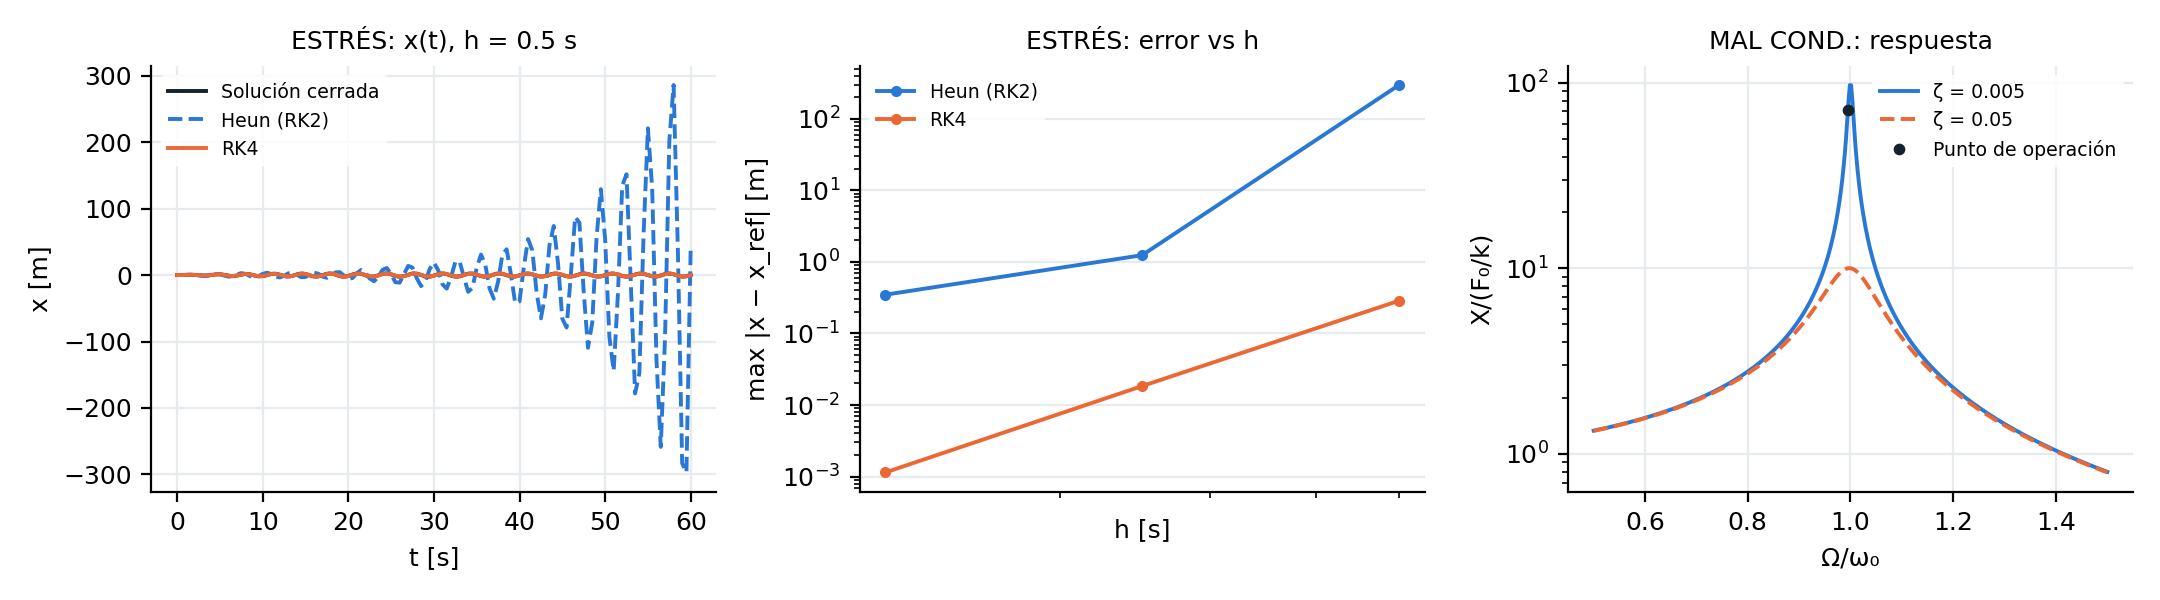
\includegraphics[width=\linewidth]{fig/s2_m3.png}
\caption{Módulo 3. Izquierda: con $h=0.5$ s Heun amplifica la oscilación ($|R|=1.051$) y RK4 no. Centro: error máximo frente a $h$. Derecha: curva de respuesta; con $\zeta=0.005$ el pico es alto y estrecho.}\end{figure}

\textbf{ESTRÉS, estabilidad y convergencia}:
{\footnotesize
\begin{longtable}{lrrrrr}
\toprule
\textbf{Método} & \textbf{h [s]} & \textbf{$\omega_{0}$h} & \textbf{|R(h$\lambda$)|} & \textbf{max |x $-$ x\_ref| [m]} & \textbf{orden p} \\
\midrule
\endhead
Heun (RK2) & 0.5 & 1 & 1.0511898 & 295.312 & — \\
Heun (RK2) & 0.25 & 0.5 & 0.98011479 & 1.23959 & 7.9 \\
Heun (RK2) & 0.125 & 0.25 & 0.98767799 & 0.347647 & 1.83 \\
RK4 & 0.5 & 1 & 0.94674369 & 0.286124 & — \\
RK4 & 0.25 & 0.5 & 0.97526711 & 0.0184104 & 3.96 \\
RK4 & 0.125 & 0.25 & 0.98757814 & 0.00114364 & 4.01 \\
\bottomrule
\end{longtable}
}

\textbf{NORMAL, refinamiento de $I$}:
{\footnotesize
\begin{longtable}{lrrrrrrr}
\toprule
\textbf{n} & \textbf{h [s]} & \textbf{Trapecio} & \textbf{Error} & \textbf{orden} & \textbf{Simpson 1/3} & \textbf{Error} & \textbf{orden} \\
\midrule
\endhead
64 & 0.3125 & 0.0247725419098 & 3.055$\times10^{-6}$ & — & 0.0247676261415 & 1.861$\times10^{-6}$ & — \\
128 & 0.15625 & 0.0247701897657 & 7.030$\times10^{-7}$ & 2.12 & 0.0247694057177 & 8.105$\times10^{-8}$ & 4.52 \\
256 & 0.078125 & 0.0247696590331 & 1.723$\times10^{-7}$ & 2.03 & 0.0247694821223 & 4.644$\times10^{-9}$ & 4.13 \\
512 & 0.0390625 & 0.0247695296196 & 4.285$\times10^{-8}$ & 2.01 & 0.0247694864818 & 2.840$\times10^{-10}$ & 4.03 \\
1024 & 0.0195312 & 0.024769497466 & 1.070$\times10^{-8}$ & 2 & 0.0247694867481 & 1.766$\times10^{-11}$ & 4.01 \\
2048 & 0.00976562 & 0.02476948944 & 2.674$\times10^{-9}$ & 2 & 0.0247694867647 & 1.102$\times10^{-12}$ & 4 \\
4096 & 0.00488281 & 0.0247694874343 & 6.685$\times10^{-10}$ & 2 & 0.0247694867657 & 6.884$\times10^{-14}$ & — \\
\bottomrule
\end{longtable}
}

\textbf{MAL CONDICIONADO, sensibilidad}: $+0.1$ \% en $\Omega$ cambia la amplitud un 10.3 \%.
{\footnotesize
\begin{longtable}{lrrrrrrr}
\toprule
\textbf{Parámetro} & \textbf{Perturbación rel.} & \textbf{X [m]} & \textbf{X' [m]} & \textbf{$\kappa$\_rel(X)} & \textbf{I} & \textbf{I'} & \textbf{$\kappa$\_rel(I)} \\
\midrule
\endhead
r & +0.001 & 0.73934151 & 0.81563614 & 103.2 & 66.616191 & 73.094187 & 97.24 \\
zeta & +0.01 & 0.73934151 & 0.73566328 & 0.4975 & 66.616191 & 65.872364 & 1.117 \\
F0 & +0.01 & 0.73934151 & 0.74673493 & 1 & 66.616191 & 67.955176 & 2.01 \\
k & +0.01 & 0.73934151 & 0.7320213 & 0.9901 & 66.616191 & 65.41855 & 1.798 \\
\bottomrule
\end{longtable}
}

\textbf{Primeras conclusiones.}
\begin{itemize}
\item \textbf{NORMAL.} \emph{Numérica:} En vibración libre RK4 reproduce la solución cerrada con error máximo 6.161$\times10^{-7}$ m y Heun con 0.00123 m; los órdenes observados se acercan a 4 y 2. Simpson y Romberg integran x$^{2}$ con muchas menos evaluaciones que el trapecio para el mismo error. \emph{Problema:} Sin viento, la oscilación inicial de 0.1 m decae con envolvente e\^{}($-\zeta\omega_{0}$t): a los 20 s queda 0.0135 m. El amortiguamiento controla cuánto dura el balanceo.
\item \textbf{ESTRÉS.} \emph{Numérica:} Con h = 0.5 s ($\omega_{0}$h = 1) Heun tiene |R(h$\lambda$)| = 1.051 > 1: amplifica la oscilación en cada paso y su error máximo llega a 295 m, mientras RK4 (|R| = 0.9467) se queda en 0.286 m. Al reducir h, Heun vuelve a ser estable y ambos recuperan sus órdenes 2 y 4. La diferencia Heun/RK4 es de estabilidad, no sólo de precisión. \emph{Problema:} La ráfaga con $\Omega$/$\omega_{0}$ = 0.95 produce una amplitud permanente de 2.296 m, 7.346 veces la deflexión estática F$_{0}$/k. Cerca de la resonancia la amplitud depende sobre todo del amortiguamiento y de la frecuencia de la ráfaga, no de la masa por sí sola. Amplitudes de ese orden superan el rango de validez de un modelo lineal de pequeñas oscilaciones.
\item \textbf{MAL COND..} \emph{Numérica:} Con $\zeta$ = 0.005 el problema es sensible: $\kappa$(X; $\Omega$) = 99, de modo que un error relativo de 0.1 \% en $\Omega$ se convierte en $\approx$ 9.9 \% en la amplitud. Numéricamente, el error de fase de Heun se acumula durante 300 s (error máx. 0.186 m) mientras RK4 queda en 1.026$\times10^{-4}$ m; ambos convergen al refinar h. La sensibilidad es del modelo, no un fallo de los métodos. \emph{Problema:} La ráfaga con $\Omega$/$\omega_{0}$ = 0.995 produce una amplitud permanente de 0.7393 m, 70.98 veces la deflexión estática F$_{0}$/k. Cerca de la resonancia la amplitud depende sobre todo del amortiguamiento y de la frecuencia de la ráfaga, no de la masa por sí sola. Amplitudes de ese orden superan el rango de validez de un modelo lineal de pequeñas oscilaciones.
\end{itemize}


% ---- M4 ----
\subsection{Módulo 4: reconstrucción de señales de sensores}
Se registran $N$ muestras uniformes de una señal conocida, se ocultan los registros $i$ con $i\bmod k=$ desfase y se reconstruyen con los restantes. NORMAL: $\sin t$ en $[0,2\pi]$; ESTRÉS: $e^{-0.3t}\sin2t$ en $[0,6]$ con ruido gaussiano $\sigma=0.002$ y semilla 7; MAL COND.: pulso de Runge $1/(1+25t^2)$ en $[-1,1]$ con 41 registros de los que se pierden los impares. Sobre el spline se busca el primer cruce de un umbral con los tres métodos de raíces; la referencia es el cruce de la señal real (bisección a $10^{-15}$).

{\footnotesize
\begin{longtable}{lrrr}
\toprule
\textbf{Parámetro} & \textbf{NORMAL} & \textbf{ESTRÉS} & \textbf{MAL COND.} \\
\midrule
\endhead
Señal sintética & seno & amortiguada & runge \\
Registros N (uniformes) & 17 & 31 & 41 \\
Ruido gaussiano $\sigma$ [u] & 0 & 0.002 & 0 \\
Semilla del ruido & 1 & 7 & 1 \\
Ocultar uno de cada k & 4 & 5 & 2 \\
Desfase de los ocultos & 2 & 2 & 1 \\
Umbral de cruce [u] & 0.5 & 0 & 0.5 \\
Tolerancia de raíces & 1.000$\times10^{-12}$ & 1.000$\times10^{-12}$ & 1.000$\times10^{-12}$ \\
\bottomrule
\end{longtable}
}

\textbf{Tabla de errores por método y escenario} (interpolación: RMS y error máximo en los ocultos, error máximo en todo el intervalo; raíces: instante de cruce):
{\footnotesize
\begin{longtable}{lllrlrrr}
\toprule
\textbf{Escenario} & \textbf{Familia} & \textbf{Método} & \textbf{Iter./pasos} & \textbf{Conv.} & \textbf{Resultado} & \textbf{Error abs.} & \textbf{Error rel. / otro} \\
\midrule
\endhead
NORMAL & Interpolación & Lagrange & 4 & sí & 2.352$\times10^{-7}$ & 3.323$\times10^{-7}$ & malla 1.172$\times10^{-6}$ \\
NORMAL & Interpolación & Newton (diferencias divididas) & 4 & sí & 2.352$\times10^{-7}$ & 3.323$\times10^{-7}$ & malla 1.172$\times10^{-6}$ \\
NORMAL & Interpolación & Spline cúbico natural & 4 & sí & 0.0011717694 & 0.00117 & malla 0.00117 \\
NORMAL & Raíces & Bisección & 31 & sí & 0.52416493 & 5.662$\times10^{-4}$ & res. 4.996$\times10^{-14}$ \\
NORMAL & Raíces & Newton-Raphson & 3 & sí & 0.52416493 & 5.662$\times10^{-4}$ & res. 0 \\
NORMAL & Raíces & Secante & 3 & sí & 0.52416493 & 5.662$\times10^{-4}$ & res. 0 \\
ESTRÉS & Interpolación & Lagrange & 6 & sí & 1.7629519 & 4.31 & malla 39.5 \\
ESTRÉS & Interpolación & Newton (diferencias divididas) & 6 & sí & 1.7629519 & 4.31 & malla 39.5 \\
ESTRÉS & Interpolación & Spline cúbico natural & 6 & sí & 0.0026865566 & 0.00533 & malla 0.00534 \\
ESTRÉS & Raíces & Bisección & 31 & sí & 1.5702137 & 5.827$\times10^{-4}$ & res. 1.673$\times10^{-13}$ \\
ESTRÉS & Raíces & Newton-Raphson & 3 & sí & 1.5702137 & 5.827$\times10^{-4}$ & res. 8.327$\times10^{-17}$ \\
ESTRÉS & Raíces & Secante & 4 & sí & 1.5702137 & 5.827$\times10^{-4}$ & res. 8.327$\times10^{-17}$ \\
MAL COND. & Interpolación & Lagrange & 20 & sí & 12.694278 & 40 & malla 59.8 \\
MAL COND. & Interpolación & Newton (diferencias divididas) & 20 & sí & 12.694278 & 40 & malla 59.8 \\
MAL COND. & Interpolación & Spline cúbico natural & 20 & sí & 0.0012684188 & 0.00317 & malla 0.00318 \\
MAL COND. & Raíces & Bisección & 29 & sí & -0.2 & 9.304$\times10^{-13}$ & res. 2.387$\times10^{-12}$ \\
MAL COND. & Raíces & Newton-Raphson & 4 & sí & -0.2 & 8.327$\times10^{-16}$ & res. 0 \\
MAL COND. & Raíces & Secante & 1 & sí & -0.2 & 8.327$\times10^{-16}$ & res. 0 \\
\bottomrule
\end{longtable}
}


\begin{figure}[h]\centering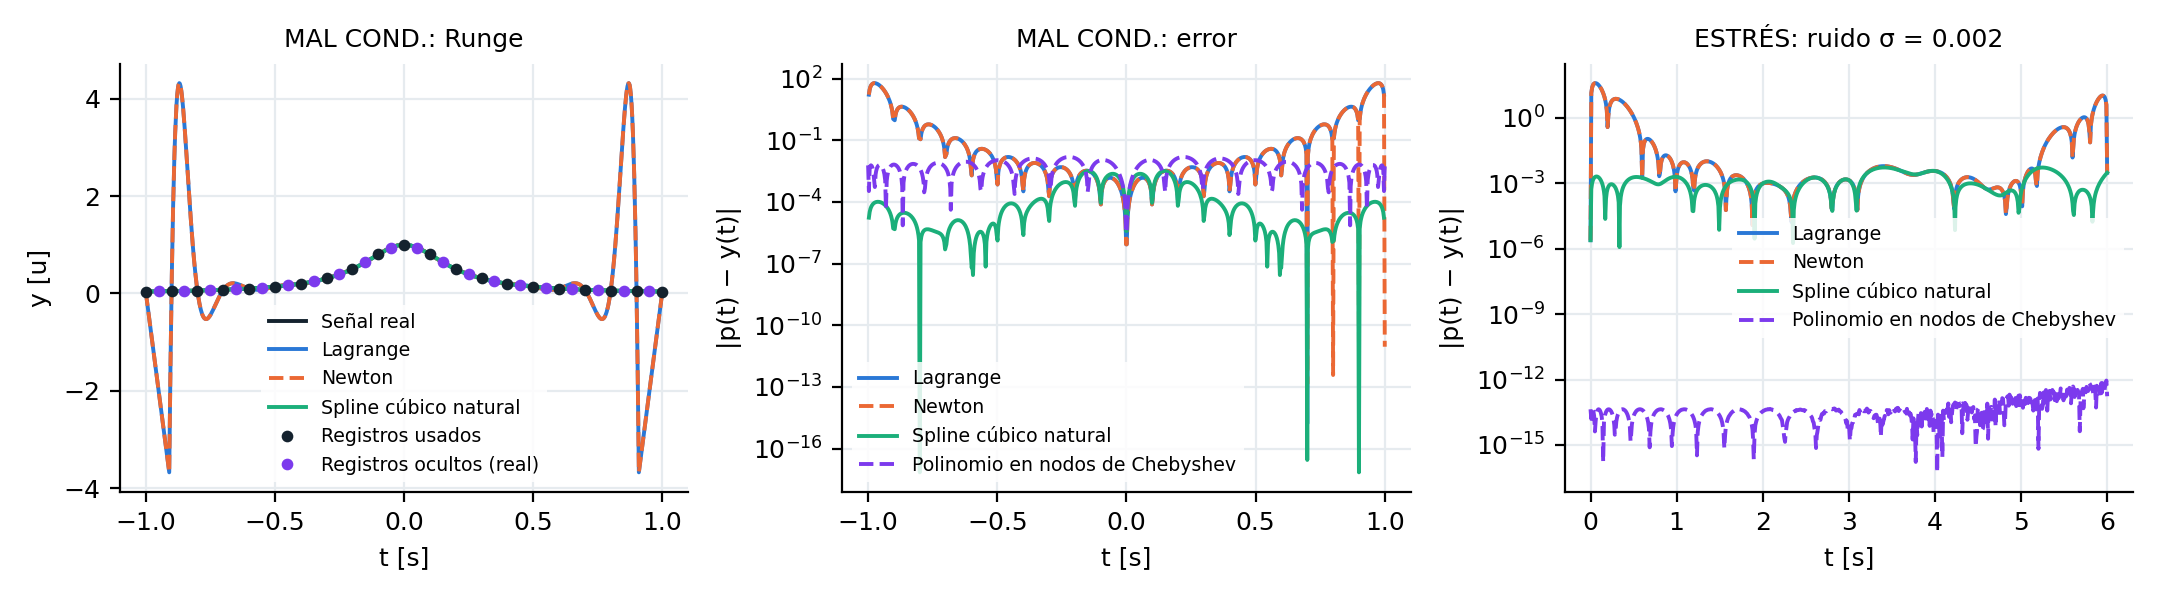
\includegraphics[width=\linewidth]{fig/s2_m4.png}
\caption{Módulo 4. Izquierda y centro: fenómeno de Runge con 21 nodos uniformes; el spline y el polinomio en nodos de Chebyshev no lo sufren. Derecha: con ruido, el polinomio de grado 24 amplifica el error hasta 39.5.}\end{figure}

\textbf{ESTRÉS, registros ocultos}:
{\footnotesize
\begin{longtable}{lrrrrrrrr}
\toprule
\textbf{i} & \textbf{t} & \textbf{y real} & \textbf{Lagrange} & \textbf{|e|} & \textbf{Newton} & \textbf{|e|} & \textbf{Spline} & \textbf{|e|} \\
\midrule
\endhead
2 & 0.4 & 0.63623778 & 4.9469579 & 4.31072 & 4.9469579 & 4.31072 & 0.63526287 & 9.749$\times10^{-4}$ \\
7 & 1.4 & 0.2201029 & 0.22938939 & 0.00928649 & 0.22938939 & 0.00928649 & 0.22079323 & 6.903$\times10^{-4}$ \\
12 & 2.4 & -0.48488537 & -0.48544438 & 5.590$\times10^{-4}$ & -0.48544438 & 5.590$\times10^{-4}$ & -0.4852532 & 3.678$\times10^{-4}$ \\
17 & 3.4 & 0.17817477 & 0.17203076 & 0.00614402 & 0.17203076 & 0.00614402 & 0.17284225 & 0.00533253 \\
22 & 4.4 & 0.15625203 & 0.15813385 & 0.00188182 & 0.15813385 & 0.00188182 & 0.15724577 & 9.937$\times10^{-4}$ \\
27 & 5.4 & -0.194126 & -0.45017464 & 0.256049 & -0.45017464 & 0.256049 & -0.19763597 & 0.00350997 \\
\bottomrule
\end{longtable}
}

\textbf{ESTRÉS, sistema auxiliar del spline}:
{\footnotesize
\begin{longtable}{lrrrrr}
\toprule
\textbf{Método} & \textbf{Iteraciones} & \textbf{¿Convergió?} & \textbf{Error relativo vs numpy.linalg.solve} & \textbf{Residuo relativo} & \textbf{t [ms]} \\
\midrule
\endhead
Gradiente conjugado & 21 & Sí & 1.615$\times10^{-14}$ & 8.875$\times10^{-15}$ & 0.406 \\
Gauss-Seidel & 22 & Sí & 2.119$\times10^{-13}$ & 7.850$\times10^{-14}$ & 2.14 \\
Jacobi & 38 & Sí & 8.594$\times10^{-14}$ & 6.464$\times10^{-14}$ & 0.635 \\
LU con pivoteo parcial & 1 & Sí & 2.958$\times10^{-17}$ & 4.030$\times10^{-17}$ & 0.485 \\
\bottomrule
\end{longtable}
}

\textbf{MAL CONDICIONADO, condicionamiento}:
{\footnotesize
\begin{longtable}{lrrrr}
\toprule
\textbf{Nodos} & \textbf{n} & \textbf{Constante de Lebesgue $\Lambda$} & \textbf{$\kappa_{2}$(Vandermonde)} & \textbf{max |p $-$ y|} \\
\midrule
\endhead
Registros disponibles & 21 & 10986.5 & 8.314$\times10^{8}$ & 59.8223 \\
Chebyshev (mismo n, remuestreo ideal) & 21 & 2.90082 & 2.306$\times10^{7}$ & 0.0153329 \\
\bottomrule
\end{longtable}
}

\textbf{NORMAL, cruce del umbral $y=0.5$} (referencia $\pi/6$):
{\footnotesize
\begin{longtable}{lrrrr}
\toprule
\textbf{Método} & \textbf{t cruce} & \textbf{Iteraciones} & \textbf{|t $-$ t\_real|} & \textbf{|s(t) $-$ u|} \\
\midrule
\endhead
Bisección & 0.524164929594 & 31 & 5.662$\times10^{-4}$ & 4.996$\times10^{-14}$ \\
Newton-Raphson & 0.524164929594 & 3 & 5.662$\times10^{-4}$ & 0 \\
Secante & 0.524164929594 & 3 & 5.662$\times10^{-4}$ & 0 \\
\bottomrule
\end{longtable}
}

\textbf{Primeras conclusiones.}
\begin{itemize}
\item \textbf{NORMAL.} \emph{Numérica:} Sin ruido y con pocos nodos, el polinomio de grado 12 es muy preciso (error 3.323$\times10^{-7}$ en los ocultos) y supera al spline (0.00117), porque sin t es analítica y sus derivadas están acotadas. Lagrange y Newton difieren sólo en 1.549$\times10^{-14}$; Newton permite agregar nodos sin recalcular todo y evaluar con Horner. \emph{Problema:} Para el sensor, la reconstrucción de los 4 registros perdidos es confiable con Newton (error máximo 3.323$\times10^{-7}$ u). El cruce del umbral se estima en t = 0.524165 s frente a 0.523599 s reales.
\item \textbf{ESTRÉS.} \emph{Numérica:} Con ruido $\sigma$ = 0.002 y grado 24, el polinomio amplifica el ruido hasta 39.5 ($\Lambda$ = 1.86$\times10^{5}$), mientras el spline lo deja en 0.00543. En los registros ocultos el spline logra 0.00533 frente a 4.31 del polinomio. El sistema del spline converge con CG, Gauss-Seidel y Jacobi por ser diagonal dominante. \emph{Problema:} Para el sensor, la reconstrucción de los 6 registros perdidos es confiable con Spline cúbico natural (error máximo 0.00533 u). Con ruido, un polinomio de grado alto no debe usarse para rellenar huecos: convierte pequeñas perturbaciones en grandes errores; el spline es la opción robusta. El cruce del umbral se estima en t = 1.57021 s frente a 1.5708 s reales.
\item \textbf{MAL COND..} \emph{Numérica:} Con 21 nodos uniformes, $\Lambda$ = 1.099$\times10^{4}$ y $\kappa_{2}$(Vandermonde) = 8.314$\times10^{8}$: el polinomio interpolante oscila cerca de los extremos (error 59.8) aunque Lagrange y Newton coinciden hasta 8.095$\times10^{-11}$. No es un fallo de los algoritmos: con nodos de Chebyshev ($\Lambda$ = 2.9) el mismo grado da 0.0153, y el spline, de grado bajo por tramos, da 0.00318. \emph{Problema:} Para el sensor, la reconstrucción de los 20 registros perdidos es confiable con Spline cúbico natural (error máximo 0.00317 u). Si el muestreo es uniforme y la señal tiene un pulso, sólo el spline (o remuestrear en nodos de Chebyshev) da una reconstrucción útil cerca de los bordes. El cruce del umbral se estima en t = -0.2 s frente a -0.2 s reales.
\end{itemize}


% ---------------- 5 ----------------
\section{Primeras comparaciones transversales}
\begin{itemize}
\item \textbf{Exactitud por grado.} En los casos polinómicos (M1 NORMAL, integración del frenado plano) los métodos son exactos hasta su grado: Heun y RK4 reproducen la parábola del frenado, Simpson integra cúbicas y Romberg quínticas. Los errores de $10^{-16}$ son redondeo, no error de método.
\item \textbf{Órdenes observados.} Heun $\to2$ y RK4 $\to4$ (M1 ESTRÉS, M3 NORMAL); trapecio $\to2$ y Simpson $\to4$ (M1 y M3); Newton cuadrático, secante $\approx1.6$–$2$ y bisección lineal en raíces simples.
\item \textbf{Estabilidad no es precisión.} En M3 ESTRÉS, con $\omega_0h=1$, Heun es inestable ($|R|>1$) y su error llega a 295 m, mientras RK4 queda en 0.29 m; al bajar a $h=0.25$ s Heun se estabiliza.
\item \textbf{Mal condicionamiento $\ne$ falta de convergencia.} En los cuatro módulos el escenario MAL CONDICIONADO se construyó como subexperimento numérico: raíz múltiple (M1), raíz casi doble y matriz de Hilbert (M2), flanco de resonancia con $\zeta$ pequeño (M3) y nodos uniformes de Runge (M4). En todos los métodos convergen (salvo Jacobi en Hilbert, por $\rho>1$, y Gauss-Seidel por $\rho\approx1$, que son propiedades del método); lo que se amplifica es el efecto de perturbaciones en los datos, medido por $\kappa$, $\Lambda$ o la amplificación observada.
\item \textbf{Residuo pequeño no implica error pequeño}, ahora fuera de los sistemas lineales: en M1 MAL COND. Newton termina con $|v|\approx10^{-50}$ y error $3\times10^{-10}$ en $t$.
\end{itemize}

% ---------------- 6 ----------------
\section{Base de datos y prueba de persistencia}
El modelo de datos conserva las 6 entidades de la semana 1. Se agregaron campos para que una simulación pueda reconstruirse sin recalcular: \texttt{simulacion.resultado\_json} (indicadores, tablas, gráficos y conclusiones, validado con \texttt{json\_valid}), \texttt{simulacion.tiempo\_total\_ms} y \texttt{ejecucion\_metodo.familia/criterio/orden}. Las iteraciones y los resúmenes siguen normalizados: una fila de \texttt{ejecucion\_metodo} por método, sus filas en \texttt{iteracion\_resultado} (como máximo 400 por método, submuestreadas de forma uniforme e incluyendo la primera y la última) y un \texttt{resultado\_resumen}. Los escenarios con los mismos parámetros se reutilizan. El historial vive en el archivo \texttt{database/simtele.db}, no en memoria.

\begin{figure}[h]\centering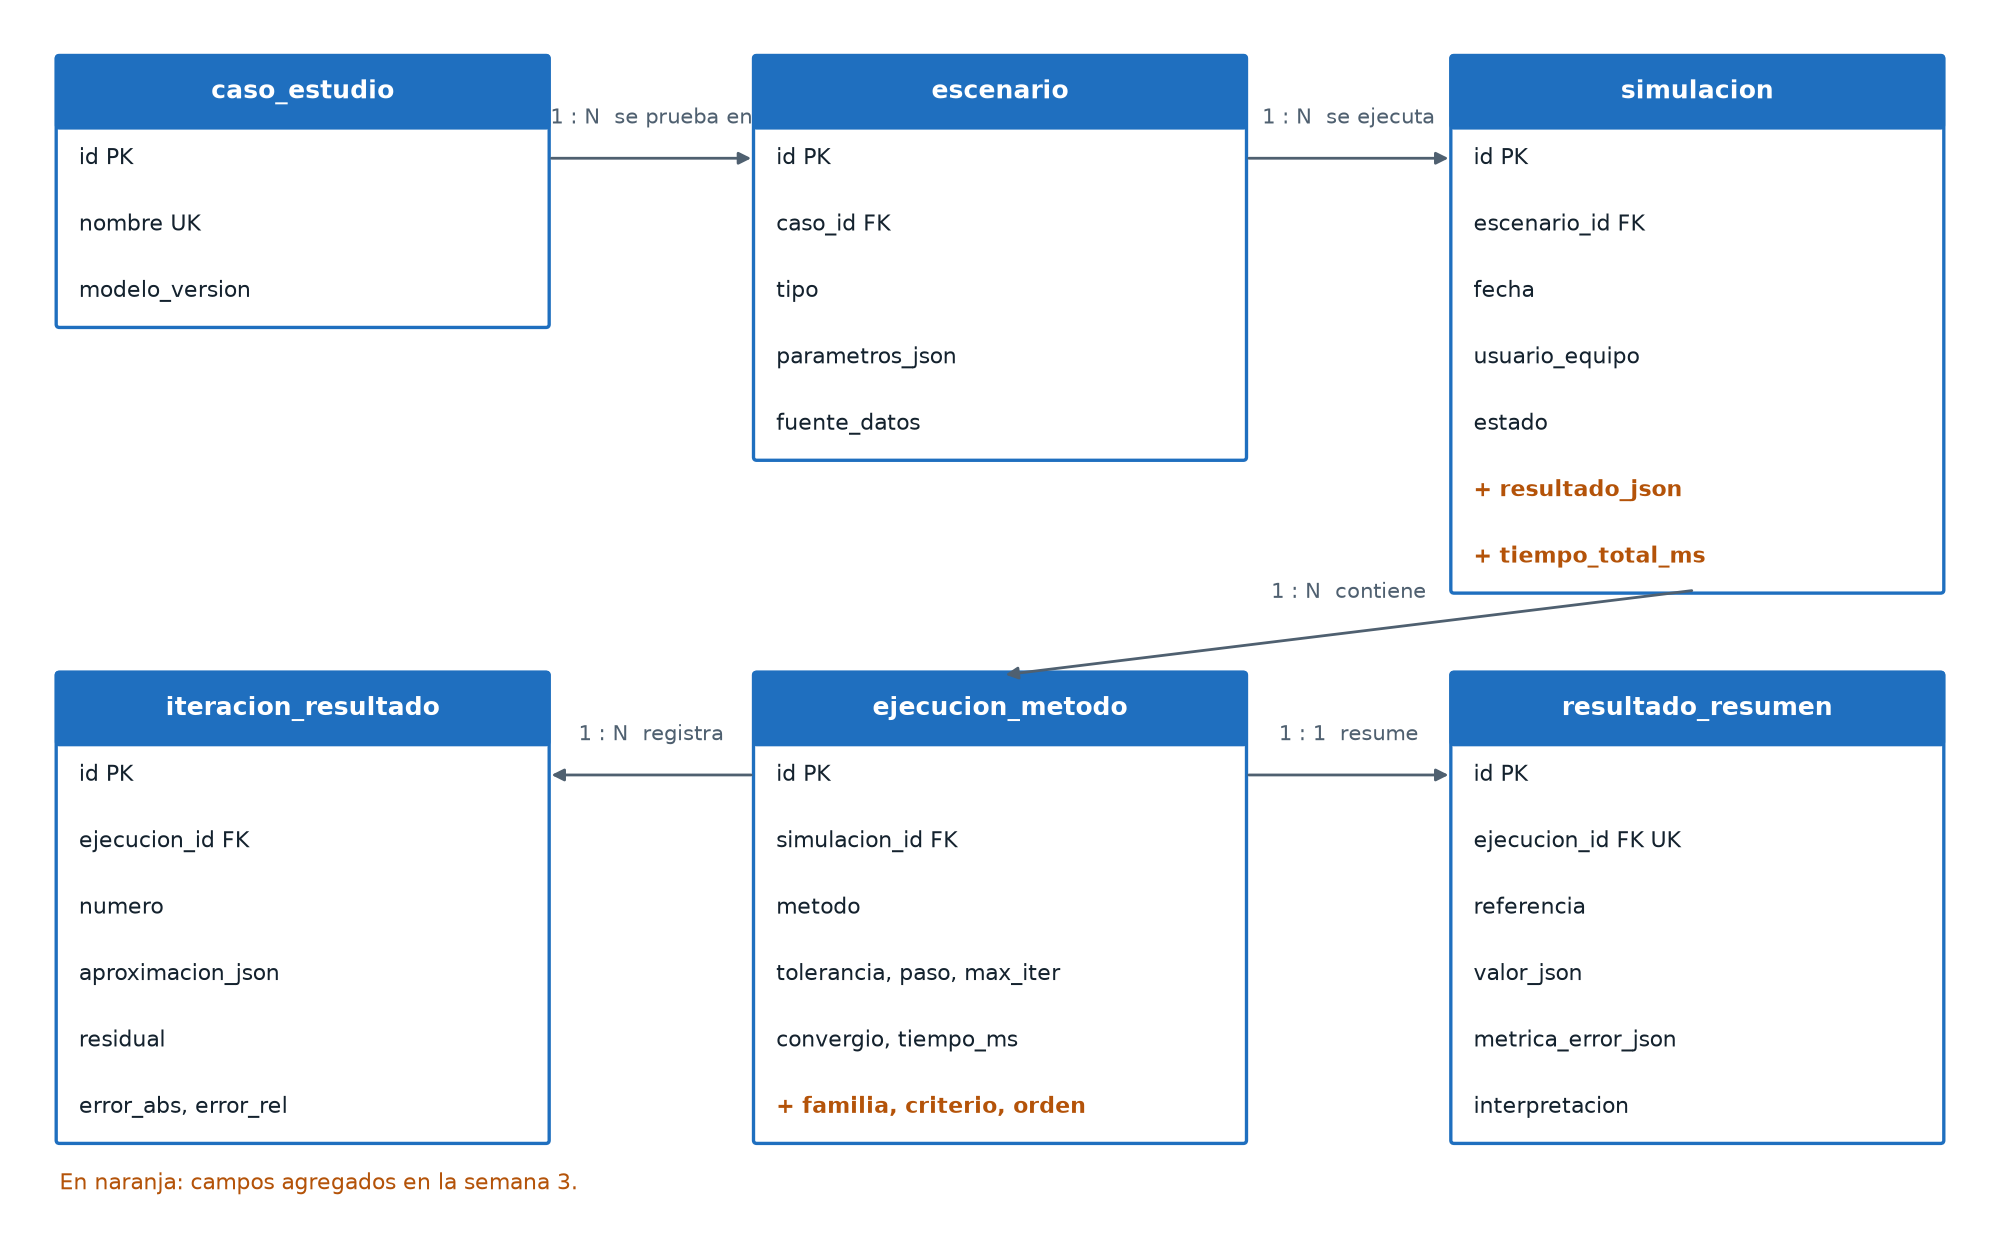
\includegraphics[width=0.92\linewidth]{fig/s2_der.png}
\caption{Modelo entidad-relación, versión 2. En naranja, los campos agregados en la semana 3.}\end{figure}

\textbf{Prueba obligatoria} (ejecutar → guardar → cerrar → recuperar → repetir → comparar). Cada simulación se guarda, se cierra la conexión, se abre una nueva, se recupera, se repite el cálculo con los parámetros recuperados y se comparan valores, métricas e iteraciones con la tolerancia $|a-b|\le10^{-12}+10^{-9}\max(|a|,|b|)$:
{\footnotesize
\begin{longtable}{rllrrrrl}
\toprule
\textbf{Sim.} & \textbf{Módulo} & \textbf{Escenario} & \textbf{Métodos} & \textbf{Filas de iteración} & \textbf{Valores comparados} & \textbf{Máx. dif. rel.} & \textbf{Coincide} \\
\midrule
\endhead
1 & M1 & ESTRÉS & 8 & 97 & 741 & 0 & sí \\
2 & M2 & MAL COND. & 7 & 611 & 7017 & 0 & sí \\
3 & M3 & NORMAL & 5 & 829 & 5776 & 0 & sí \\
4 & M4 & ESTRÉS & 6 & 56 & 452 & 0 & sí \\
\bottomrule
\end{longtable}
}

La misma prueba se automatizó en \texttt{test\_guardar\_cerrar\_recuperar\_y\_repetir} y \texttt{test\_api\_extremo\_a\_extremo}, y se verificó en la aplicación reiniciando el servidor: la simulación \#1 (M2, MAL COND.) se recuperó y relanzó con 7017 valores coincidentes. Una prueba adicional comprueba que la comparación sí detecta un cambio relativo de $10^{-6}$.

% ---------------- 7 ----------------
\section{Experimentos y fallos detectados}
\subsection{Fallos de los métodos observados en los experimentos}
{\small
\begin{longtable}{p{3.2cm}p{5.6cm}p{6.4cm}}
\toprule
\textbf{Dónde} & \textbf{Observación} & \textbf{Causa e interpretación}\\
\midrule
M3 ESTRÉS, Heun & Error máximo de 295 m con $h=0.5$ s. & $|R(h\lambda)|=1.051>1$: inestabilidad numérica, no física. Con $h\le0.25$ s desaparece.\\
M2 MAL COND., Jacobi & Diverge en 128 iteraciones. & $\rho(T_J)=6.04>1$ con Hilbert.\\
M2 MAL COND., Gauss-Seidel & No termina en 5000 iteraciones. & $\rho(T_{GS})\approx1$: converge en teoría pero muy lento.\\
M1 MAL COND., EDO & $t_{\mathrm{det}}$ con error de 0.11 s (RK4) y 1.0 s (Heun). & Raíz de multiplicidad 5; orden observado $p/5$.\\
M1 MAL COND., Newton y secante & 104 y 146 iteraciones. & Convergencia lineal (razón $4/5$) en raíz múltiple.\\
M2 MAL COND., raíces & $+10^{-7}$ relativo en $D_u$ elimina la raíz. & $D'(t^*)\approx4.5\times10^{-4}$: curva casi tangente.\\
M4 ESTRÉS, polinomio & Error 39.5 con datos de error 0.002. & $\Lambda=1.9\times10^5$ con 25 nodos uniformes y huecos.\\
M4 MAL COND., polinomio & Error 59.8 cerca de los extremos. & Fenómeno de Runge; nodos de Chebyshev bajan el error a 0.015.\\
\bottomrule
\end{longtable}}

\subsection{Fallos de implementación encontrados y corregidos}
\begin{enumerate}
\item \textbf{Detención con paso fijo.} Integrar con paso fijo hasta que $v<0$ sobrepasa la detención y deja velocidad negativa. Se reemplazó por el ajuste del último paso $h^*$ con la secante (bisección de respaldo), lo que hace exacto el caso de desaceleración constante.
\item \textbf{Romberg sobre la salida de RK4.} Romberg necesita $2^j$ subintervalos; con $N=400$ sólo caben 5 niveles. Se implementó \texttt{romberg\_datos}, que usa los trapecios con pasos $h\,2^j$ disponibles.
\item \textbf{Simpson con $n$ impar.} Las mallas de RK4 recortadas pueden tener $n$ impar; se agregó Simpson 3/8 en el último tramo para conservar el orden 4.
\item \textbf{Errores relativos con referencia nula} ($x(0)=0$, cruces por cero): se omiten en lugar de dividir por cero; los gráficos logarítmicos excluyen errores exactamente nulos y lo advierten.
\item \textbf{Esquema SQL.} Las nuevas columnas rompían los \texttt{INSERT} posicionales de la prueba del esquema; se reescribieron con columnas nombradas y se agregó una prueba de \texttt{json\_valid}.
\item \textbf{Compatibilidad.} Una f-string anidada con comillas iguales sólo funcionaba en Python $\ge3.12$; se reescribió para mantener la compatibilidad con Python 3.10 declarada en el README.
\item \textbf{Escala de gráficos.} El polinomio de Runge alcanza $\pm60$ y aplastaba la escala; en la curva reconstruida se recortan los valores con $|p|>5$ y se indica en la nota del gráfico.
\end{enumerate}

\subsection{Pendiente para la semana 3}
\begin{enumerate}
\item Validar con los datos de referencia los tres escenarios de los cuatro casos y completar las comparaciones con gráficos de error y convergencia.
\item Redactar las conclusiones definitivas (numérica y del problema) de cada caso y la conclusión integradora.
\item Publicar la aplicación con persistencia, grabar el video de 3 minutos y preparar la defensa: cada integrante cambia parámetros, ejecuta, recupera un experimento y lo interpreta.
\end{enumerate}

% ---------------- 8 ----------------
\section{Enfoque por mención}
{\small
\begin{longtable}{p{2.6cm}p{12.6cm}}
\toprule
\textbf{Mención} & \textbf{Aporte en la semana 3}\\
\midrule
Ingeniería de Sistemas & API REST con validación y errores 422, persistencia transaccional en SQLite y recuperación sin recalcular, prueba de reinicio, aplicación web con historial y modo estático, 33 pruebas nuevas (de 21 a 54).\\
IA y Ciencia de Datos & Diseño de los escenarios con datos sintéticos reproducibles (semillas, ruido controlado), validación con registros ocultos, constante de Lebesgue y amplificación del ruido, métricas de error y sensibilidad en los cuatro módulos.\\
\bottomrule
\end{longtable}}

\section*{Referencias}
\begin{itemize}
\item Burden, R. L. y Faires, J. D. \emph{Análisis numérico}.
\item Chapra, S. C. y Canale, R. P. \emph{Métodos numéricos para ingenieros}.
\item Golub, G. H. y Van Loan, C. F. \emph{Matrix Computations}.
\item Trefethen, L. N. \emph{Approximation Theory and Approximation Practice} (nodos de Chebyshev y constante de Lebesgue).
\end{itemize}

\end{document}
